% Пример заготовки для презентации с использованием класса Beamer LaTeX.
% Версия от 09 ноября 2018 года.
\documentclass[12pt,a4paper,mathserif]{beamer}
\usepackage[utf8x]{inputenc}
\usepackage{ucs}
\usepackage[T2A]{fontenc}
\usepackage[english,russian]{babel}
\usepackage{amsmath}
\usepackage{amsfonts}
\usepackage{amssymb}
\usepackage{mathtext}
\usepackage{graphicx}
\usepackage{enumerate}
\usepackage{multirow}
\usepackage{ragged2e}
% Пакет для оформления исходного кода
\usepackage{minted}
\usepackage{adjustbox}
\justifying
\renewcommand{\raggedright}{\leftskip=0pt \rightskip=0pt plus 0cm}
\setbeamertemplate{caption}[numbered]

\usetheme {Madrid}
\usecolortheme [RGB={75, 0, 130}]{structure} %Dark Olive Green

\author[Laptev A.V.]{{Student of group 595: Laptev A.~V.}\\
{Scientific supervisor: Shmakov I.~A.}}
\title[Barnaul 2023]{Development and development of a device for generating a character D\&D}
% \subtitle{Отчет по научно-исследовательской работе}

\begin{document}
\begin{frame}
\maketitle
\end{frame}

\begin{frame}{Relevance}
    \setlength{\parindent}{0.5cm}
    To date, D\&D is perhaps the most popular strategy that has gathered a huge community of players around it.

    To play this table role -playing game, each player must create his own character with certain skills and characteristics. The creation of the character is a rather long and painstaking process that requires the knowledge of the rules of the game, which are quite extensive. This device is necessary in order to facilitate players, especially beginners, the generation of their game character and perform most of the calcula-\ tions of game characteristics instead of players.
    
     For D\&D, a huge number of Web resources and bots have been developed from enthusiasts and large companies that make the players the process of playing and generating their character.
\end{frame}

\begin{frame}{The purpose and objectives of scientific work}
    \setlength{\parindent}{0.5cm}
    The aim of the work is: to design and develop a portable device for generating a character D\&D, which will be adapted for everyday use anywhere without connecting to the Internet.

     Tasks that need to be solved to achieve the goal:

    \begin{enumerate}
        \item selection of components necessary for prototyping;
        
        \item design of the functionality of the application;
        
        \item Implementation in the software code of algorithms according to the basic rules D\&D5;
        
        \item debugging and testing of the software and hardware part of the prototype of the device;
        
        \item Assembly of the prototype of the device.
    \end{enumerate}
\end{frame}

\begin{frame}{The functionality of the character generator}
    \setlength{\parindent}{0.5cm}
    The necessary functionality implemented in this generator of the characters:

    \begin{enumerate}
        \item the choice of character race;
    
        \item the choice of class race;
    
        \item Generation of values of 5 basic characteristics:
    
        \begin{enumerate}
            \item strong --- abbreviated <<Str>>;
            
            \item constitution --- abbreviated <<Con>>;
            
            \item dexterity --- abbreviated <<Dex>>);
            
            \item intelligence --- abbreviated <<Int>>);
            
            \item wisdom --- abbreviated <<Wis>>);
            
            \item charisma --- abbreviated <<Cha>>).
        \end{enumerate}
    
        \item Calculation of values for a number of side effects: a class of defense and a characteristic character (based on basic characteristics).
    
        % \item Выбор снаряжения на основе ранее выбранных игроком характеристик;
    
        % \item Еще некоторые побочные характеристики.
    \end{enumerate}
\end{frame}

\begin{frame}{\small Selection of the hardware. Choosing a debug}
    \tiny
    \begin{minipage}{0.5\linewidth}
    ATmega328:
    \begin{itemize}
        \item MCU: ATmega328;
        \item clock frequency: 16 MHz;
        \item the voltage of logical levels: 5 V;
        \item input voltage of the supply: 7-12 V;
        \item general-purpose input and output ports: 20;
        \item maximum current with input-output: 40 mA;
        \item maximum output current pin 3.3V: 50 mA;
        \item maximum output current pin 5V: 800 mA;
        \item ports with PWM support: 6;
        \item ports with ADC: 6;
        \item the discharge of ADC: 10 bit;
        \item flash-memory: 32 Kb;
        \item EEPROM-memory: 1 Kb;
        \item RAM: 2 Kb;
        \item sizes: 69×53 mm.
    \end{itemize}
    \end{minipage}
    \hfill
    \begin{minipage}{0.5\linewidth}
    Xtensa LX6:
    \begin{itemize}
        \item MCU: Xtensa LX6;
        \item clock frequency: 160-240 MHz;
        \item the voltage of logical levels: 3,3 V;
        \item вхоinput voltage of the supply: 5-14 V;
        \item general-purpose input and output ports: 10;
        \item maximum current with input-output: 12 mA;
        \item maximum output current pin 3.3V: 1 А;
        \item порты с поддержкой ШИМ: 16;
        \item ports with ADC: 18;
        \item the discharge of ADC: 12 bit;
        \item flash-memory: 448 КБ;
        \item RAM: 520 КБ;
        \item wireless network: Wi-fi 802.11 b/g/n 2.4 Hz (150 Mb/sec);
        \item Bluetooth: v4.2 BR/EDR and BLE;
        \item sizes: 51x28 mm.
    \end{itemize}
    \end{minipage}
\end{frame}

\begin{frame}{\small Selection of the hardware. The choice of periphery}
    \scriptsize
    \begin{minipage}{0.5\linewidth}
    1602 LCD Keypad Shield:
    \begin{itemize}
        \item brightness color: blue;
        \item the number of characters in the line: 16;
        \item number of lines: 2;
        \item language: latin;
        \item compatible with Arduino Uno;
        \item supply voltage: 5 V;
        \item type of display matrix: LCD;
        \item 5 buttons for control and discharge button.
    \end{itemize}
    \end{minipage}
    \hfill
    \begin{minipage}{0.5\linewidth}
    LCD-display:
    \begin{itemize}
        \item brightness color: blue;
        \item the number of characters in the line: 16;
        \item number of lines: 2;
        \item language: latin;
        \item еo connect you need a maket board;
        \item supply voltage: 5 V;
        \item type of display matrix: LCD;
    \end{itemize}
    Кнопки:
    \begin{itemize}
        \item 5 buttons for control and discharge button;
        \item еo connect you need a maket board.
    \end{itemize}
    \end{minipage}
\end{frame}

\begin{frame}{The appearance of the device}
    \begin{figure}[H]
        \begin{minipage}[h]{0.45\linewidth}
            \center{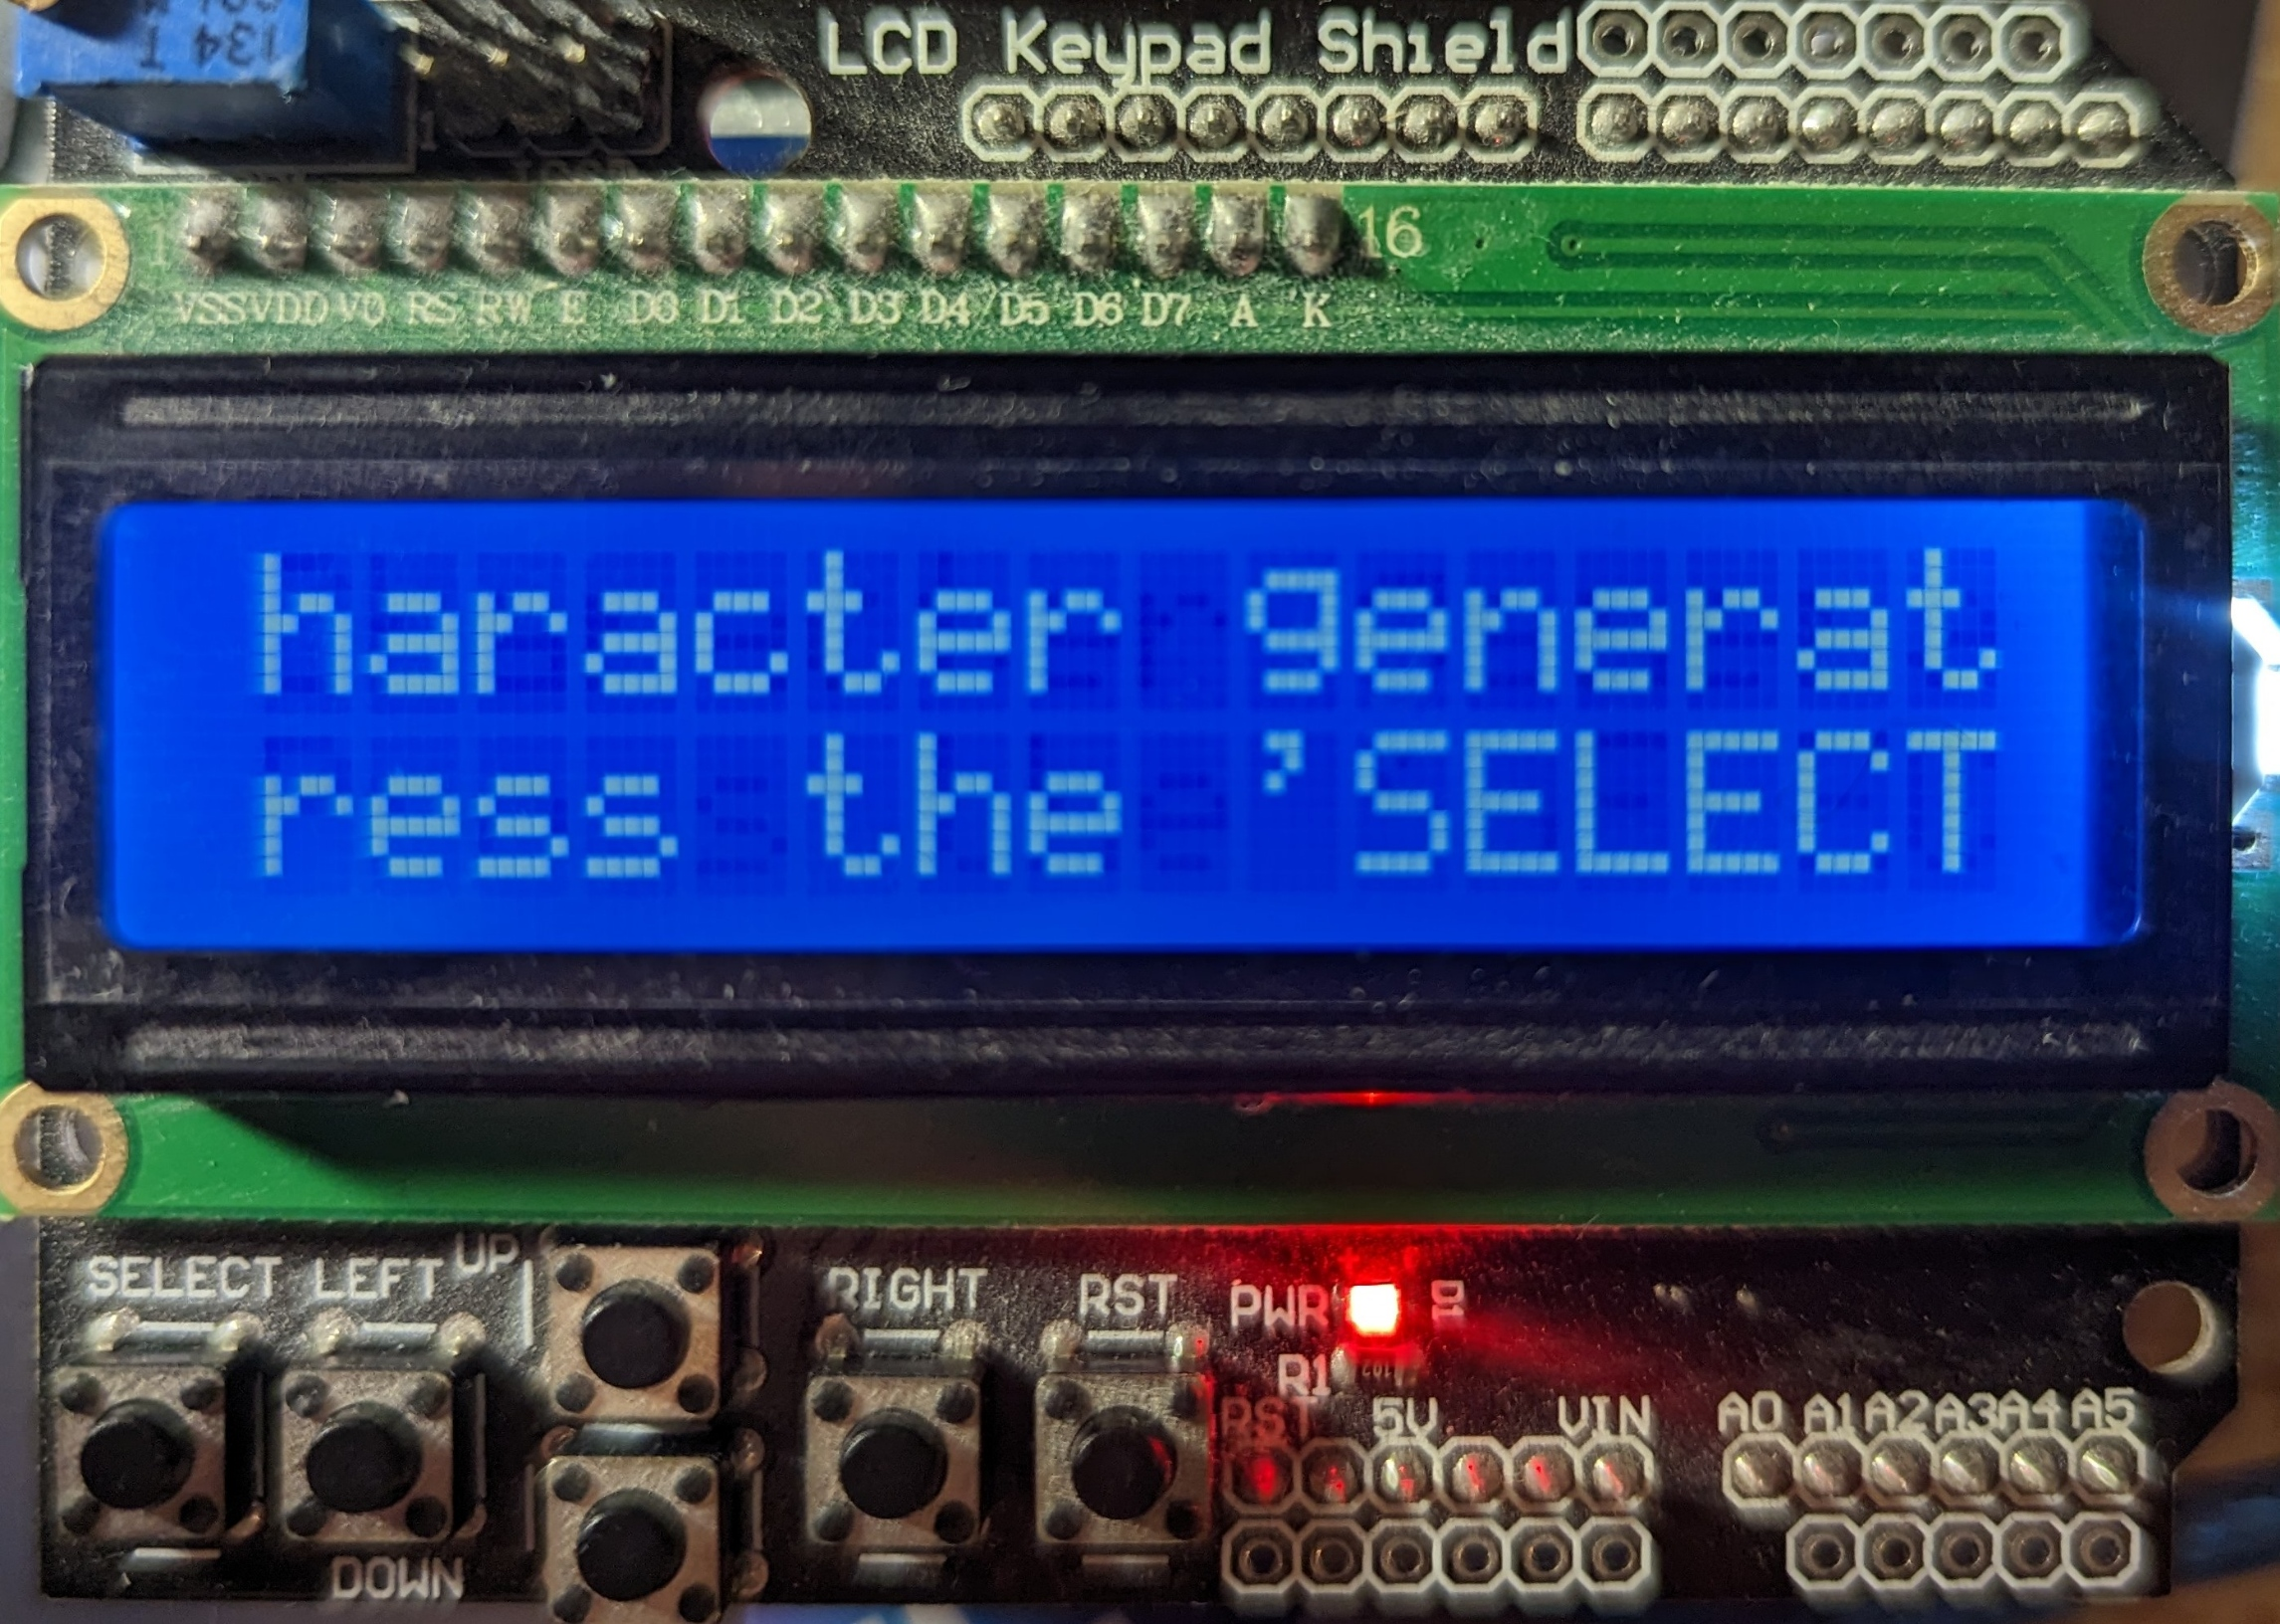
\includegraphics[width=1\linewidth]{mainWindow.jpg}} \\
        \end{minipage}
        \hfill
        \begin{minipage}[h]{0.45\linewidth}
            \center{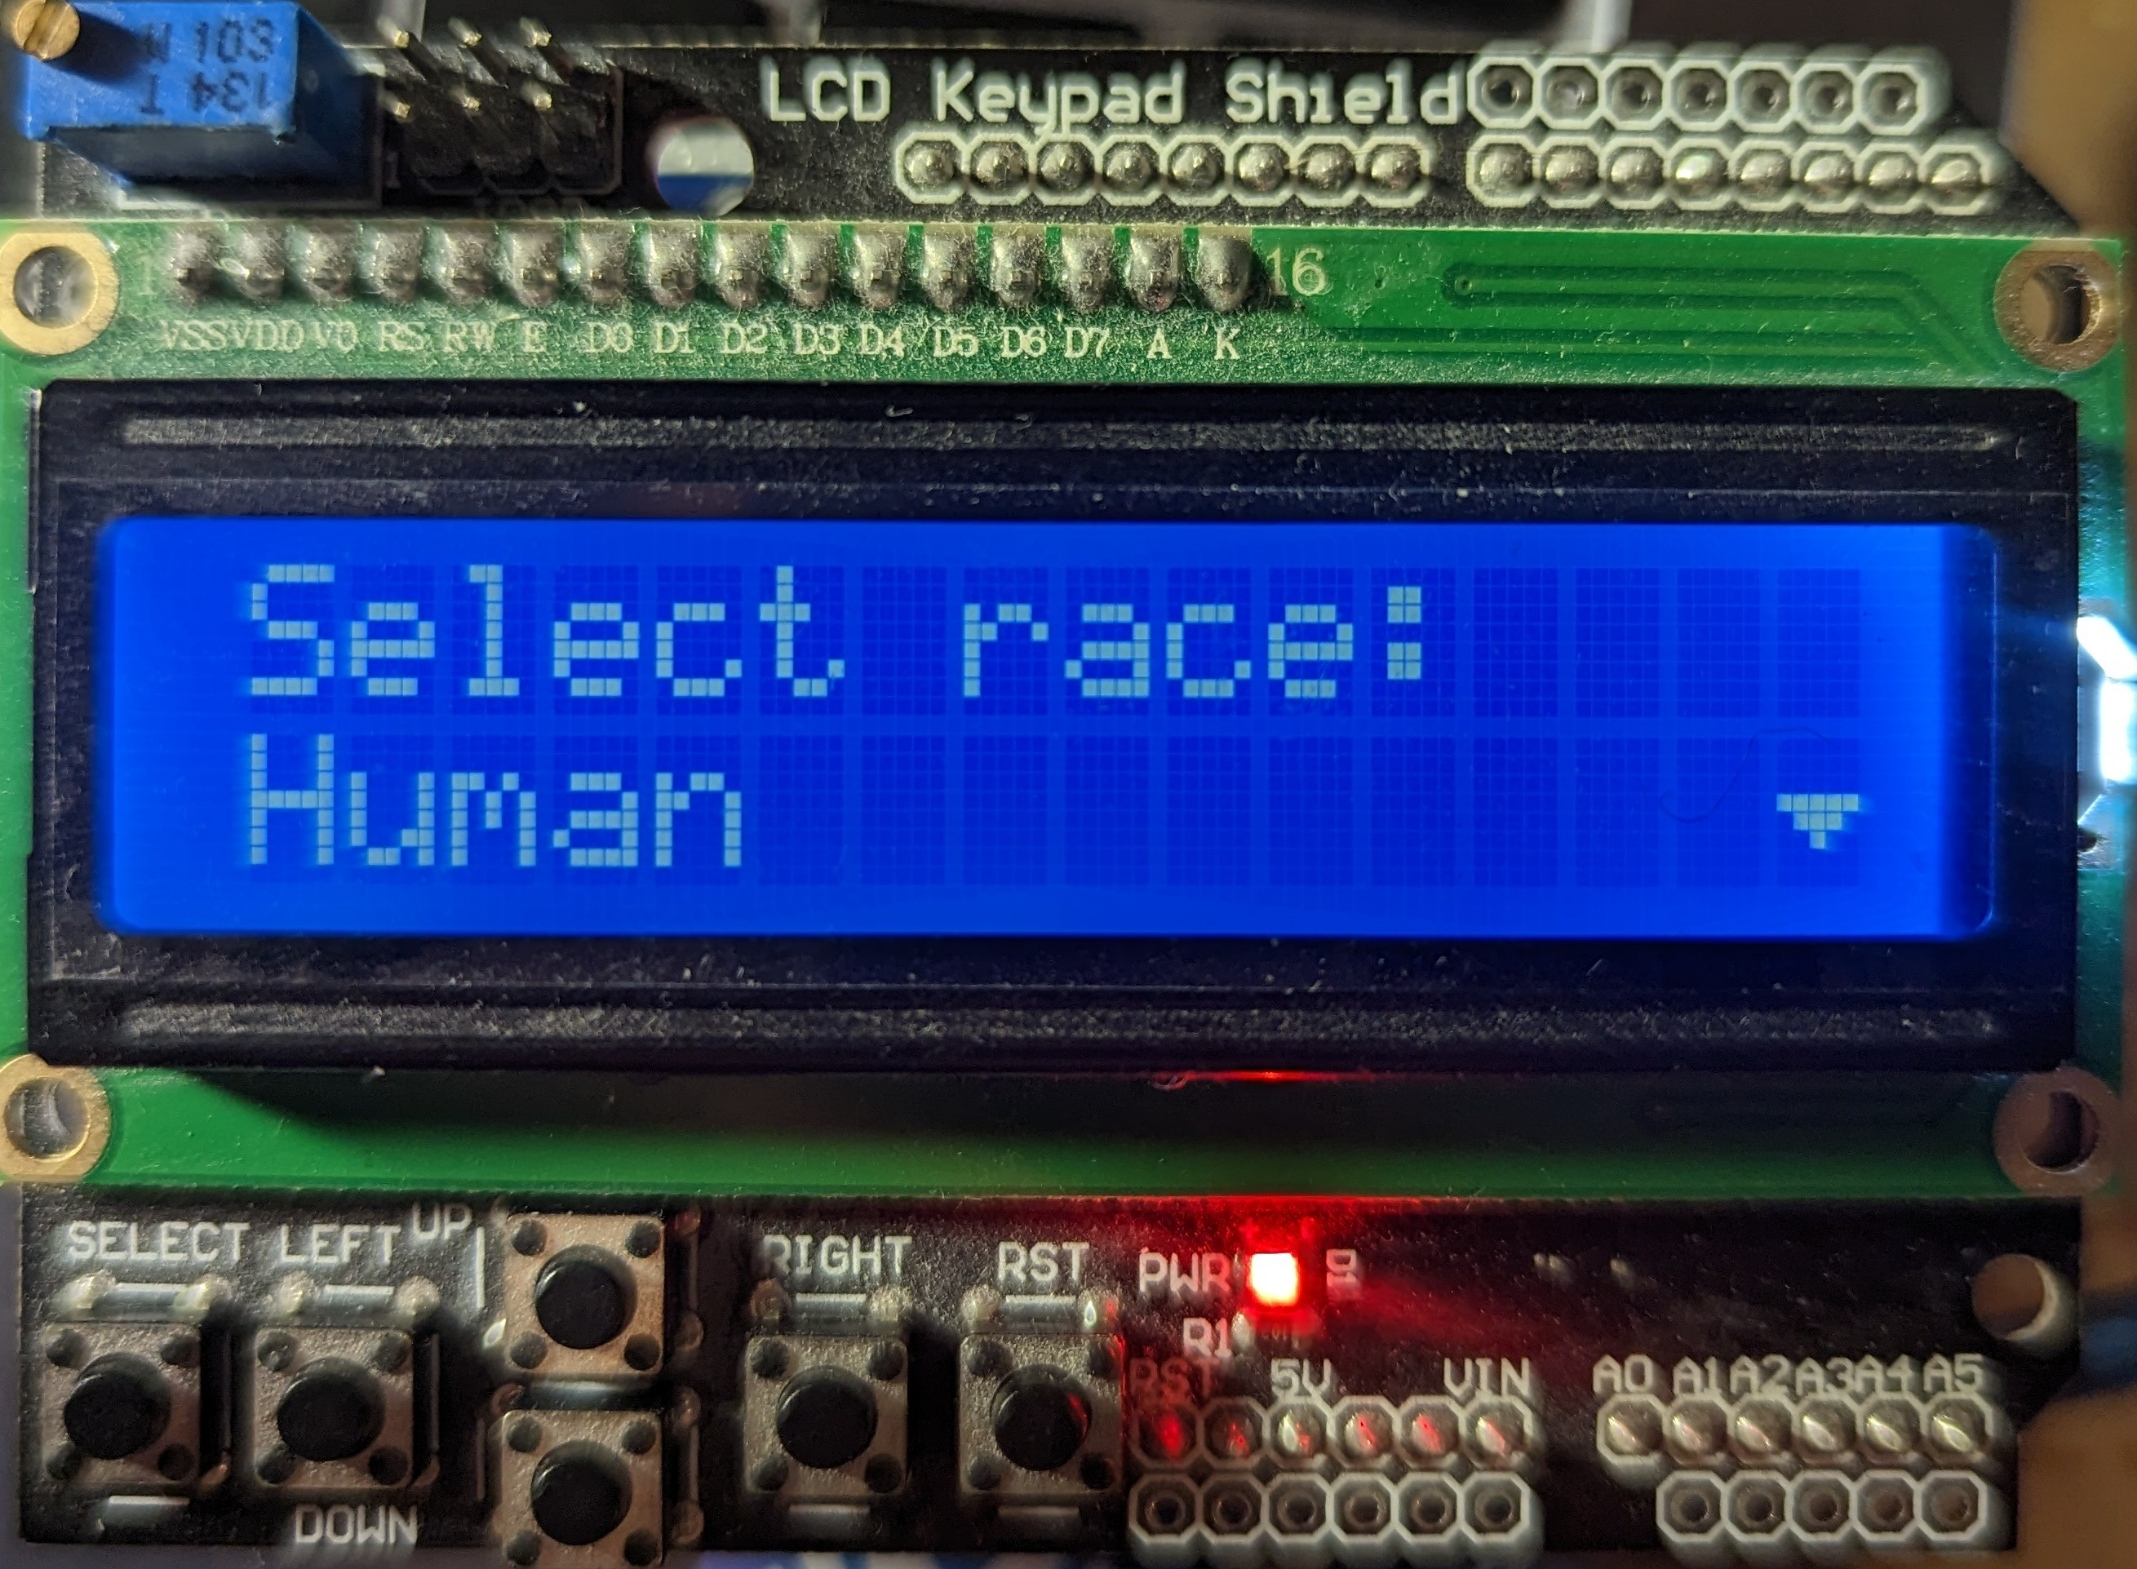
\includegraphics[width=1\linewidth]{selectRace.jpg}} \\
        \end{minipage}
        \vfill
        \begin{minipage}[h]{0.45\linewidth}
            \center{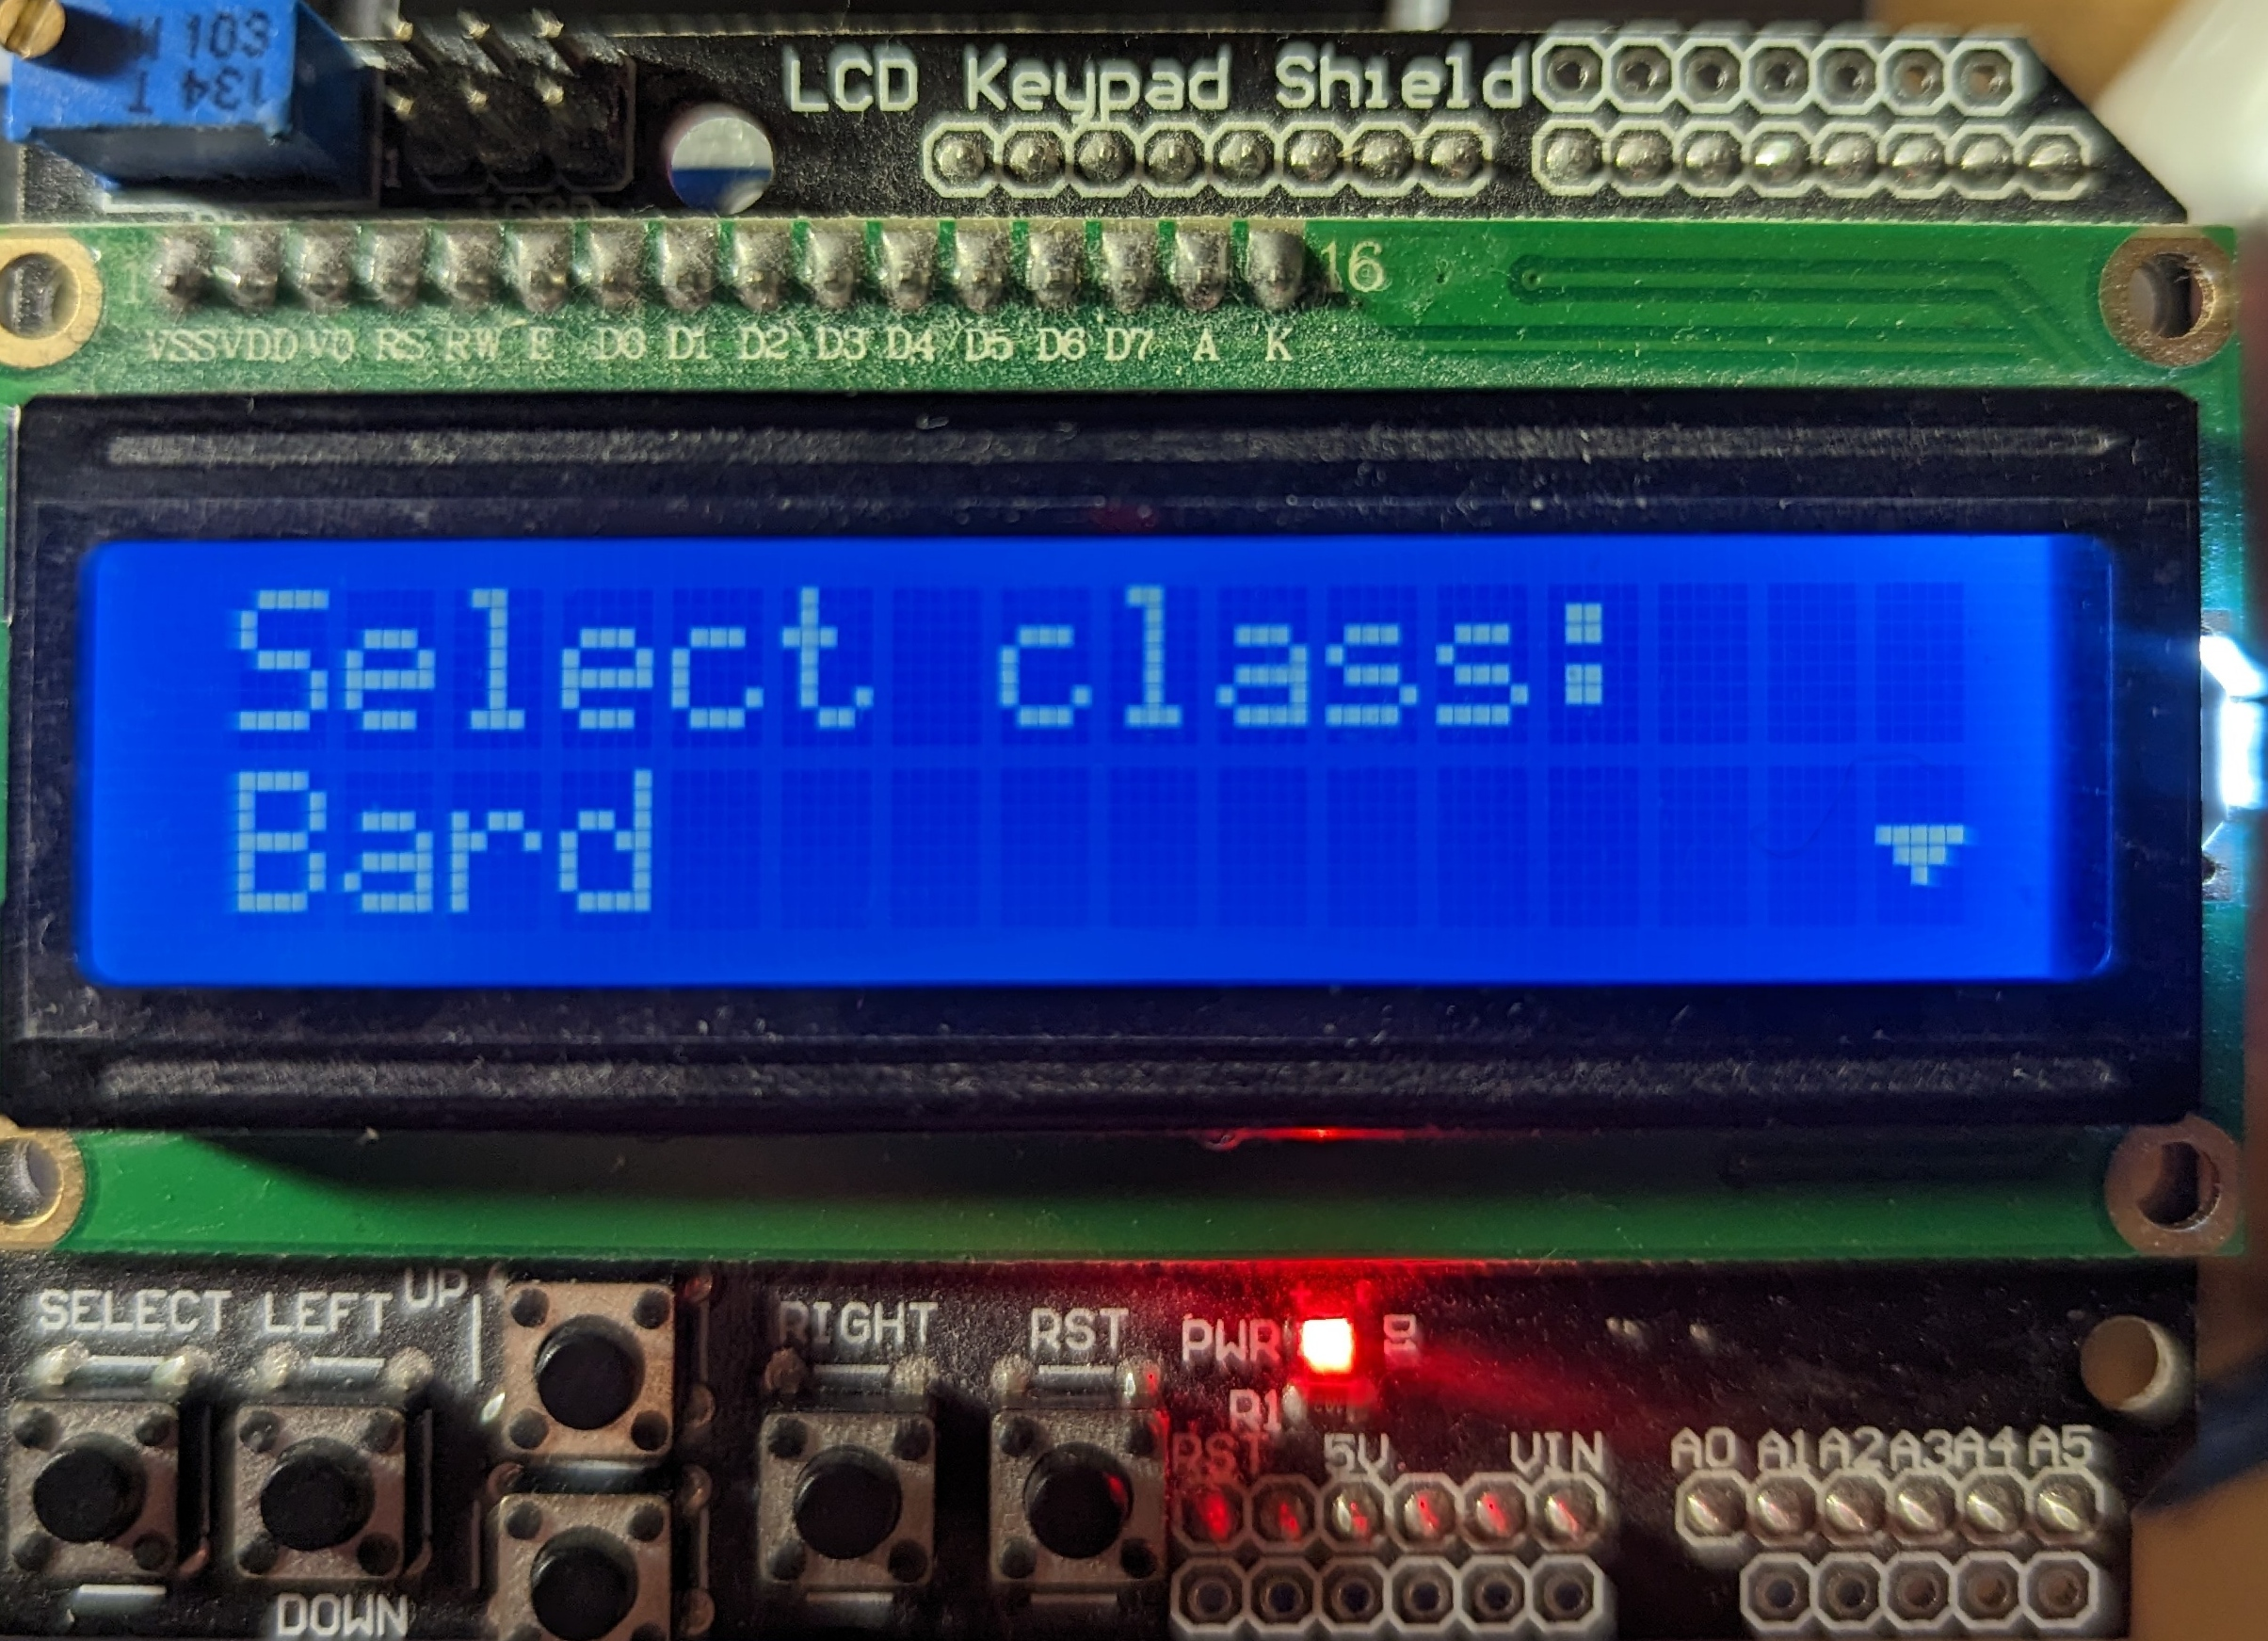
\includegraphics[width=1\linewidth]{selectClass.jpg}} \\
        \end{minipage}
        \hfill
        \begin{minipage}[h]{0.45\linewidth}
            \center{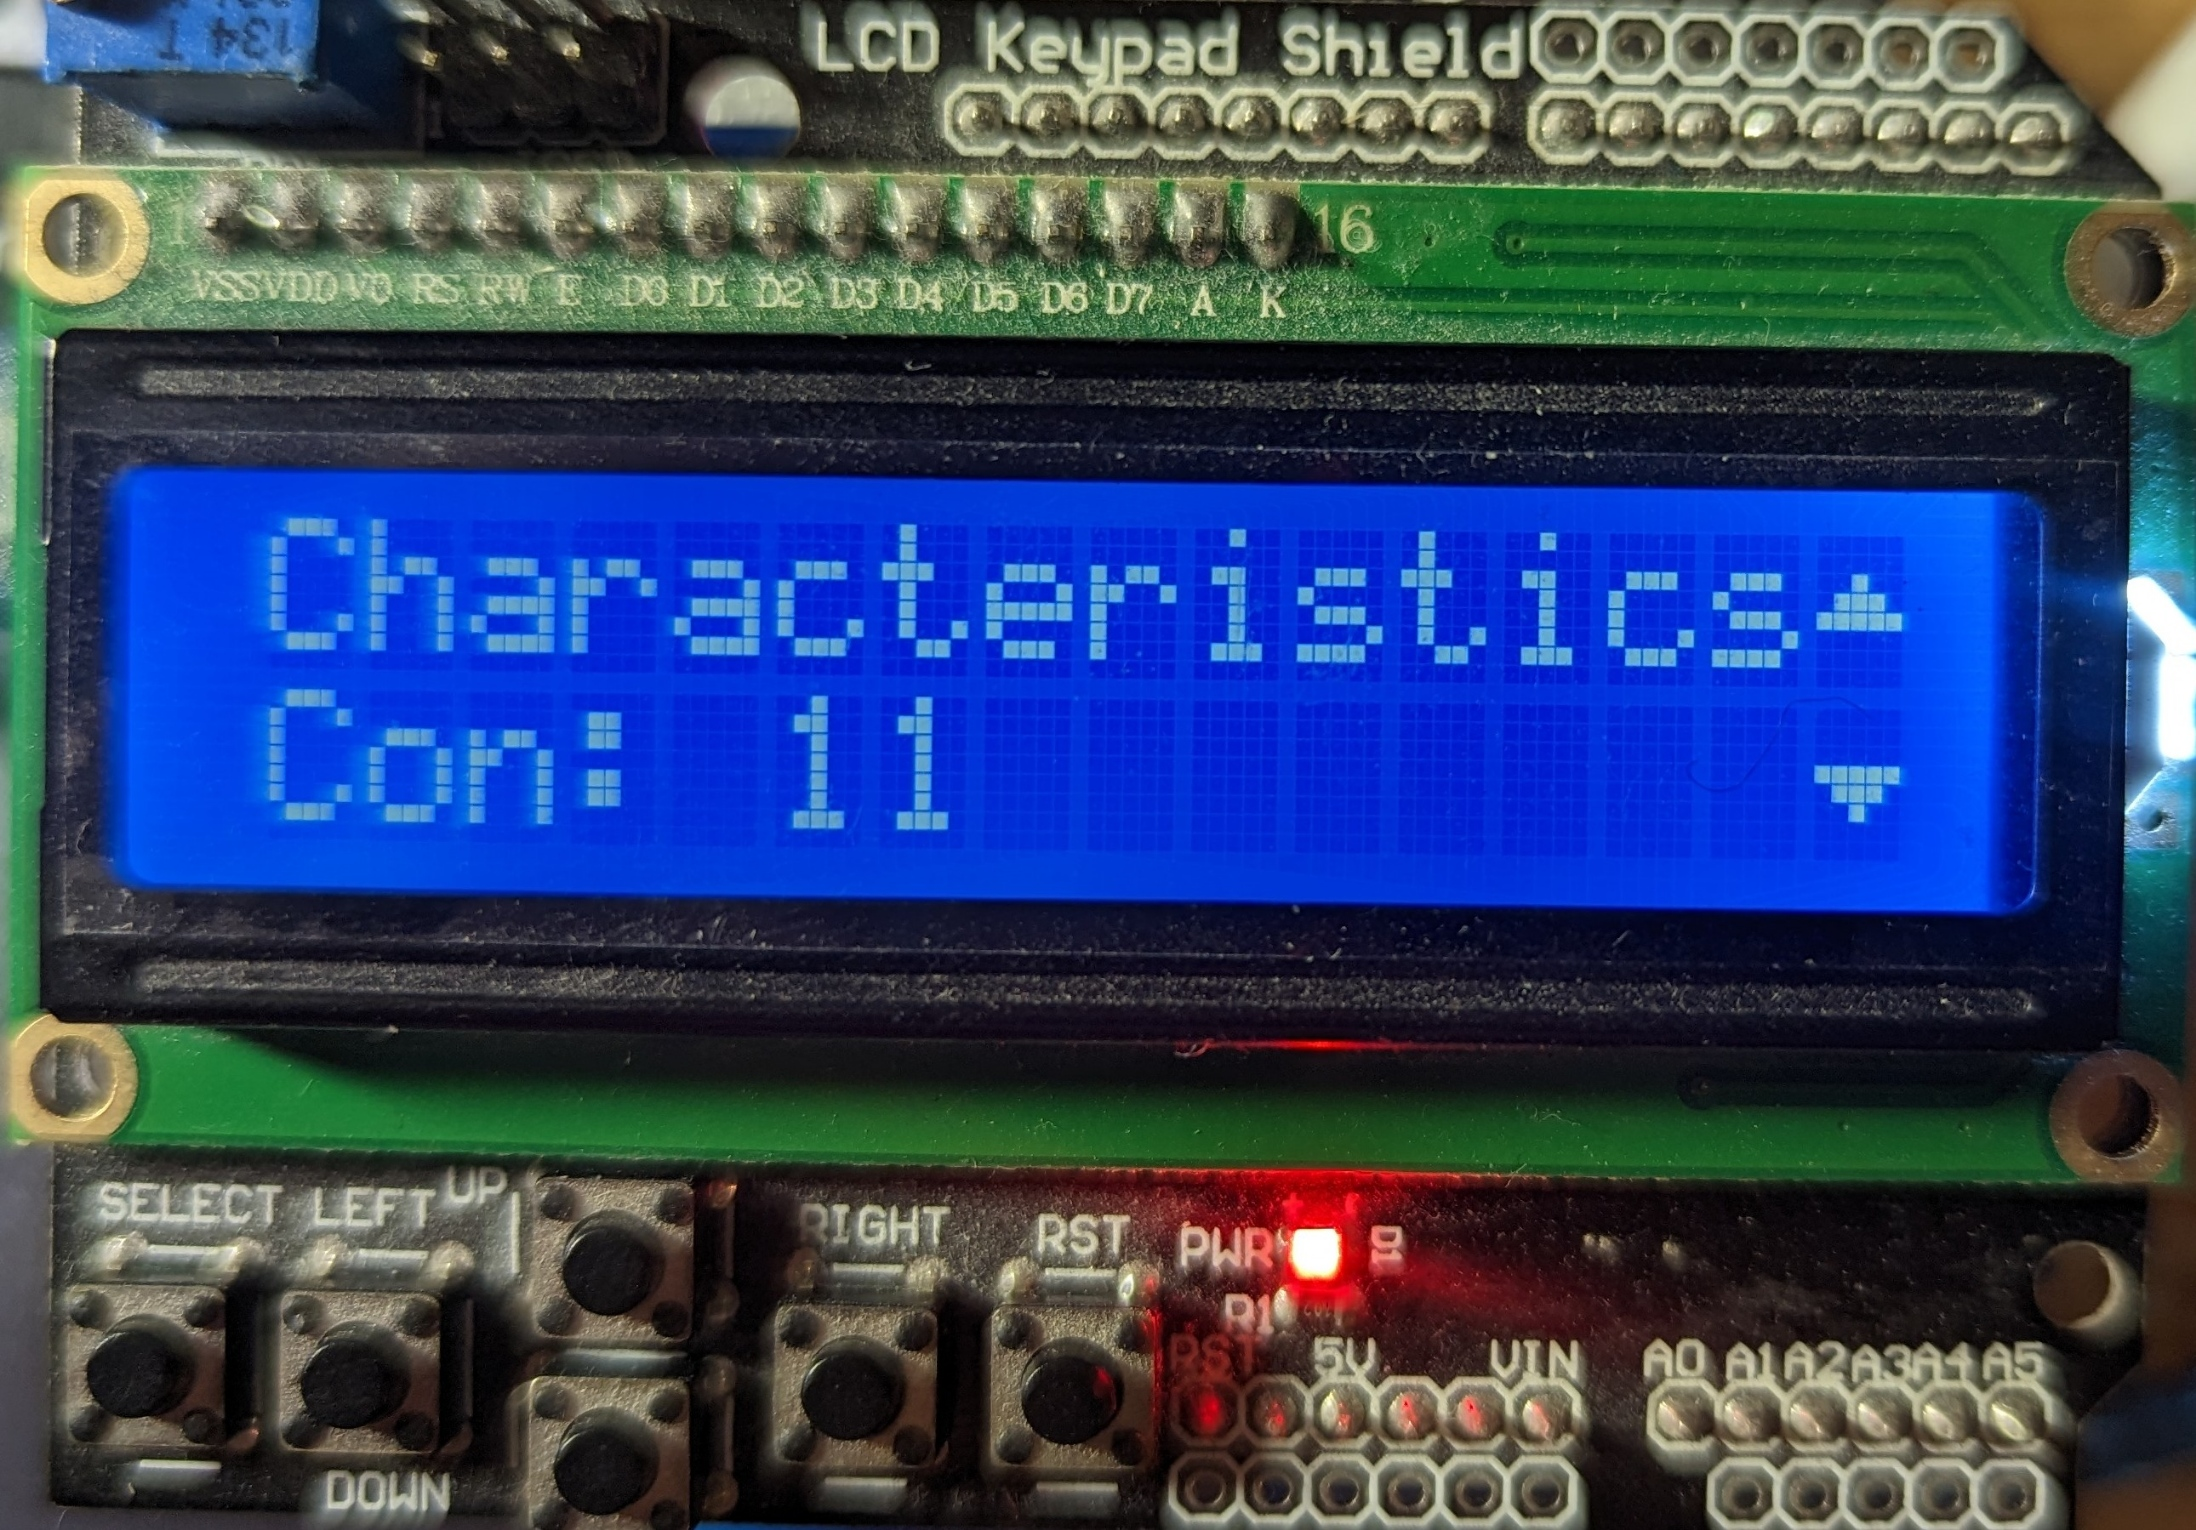
\includegraphics[width=1\linewidth]{output.jpg}} \\
        \end{minipage}
    \end{figure}
\end{frame}

\begin{frame}[fragile]{{\small Block diagram algorithm for choosing a character race}}
\begin{figure}
        \centering
        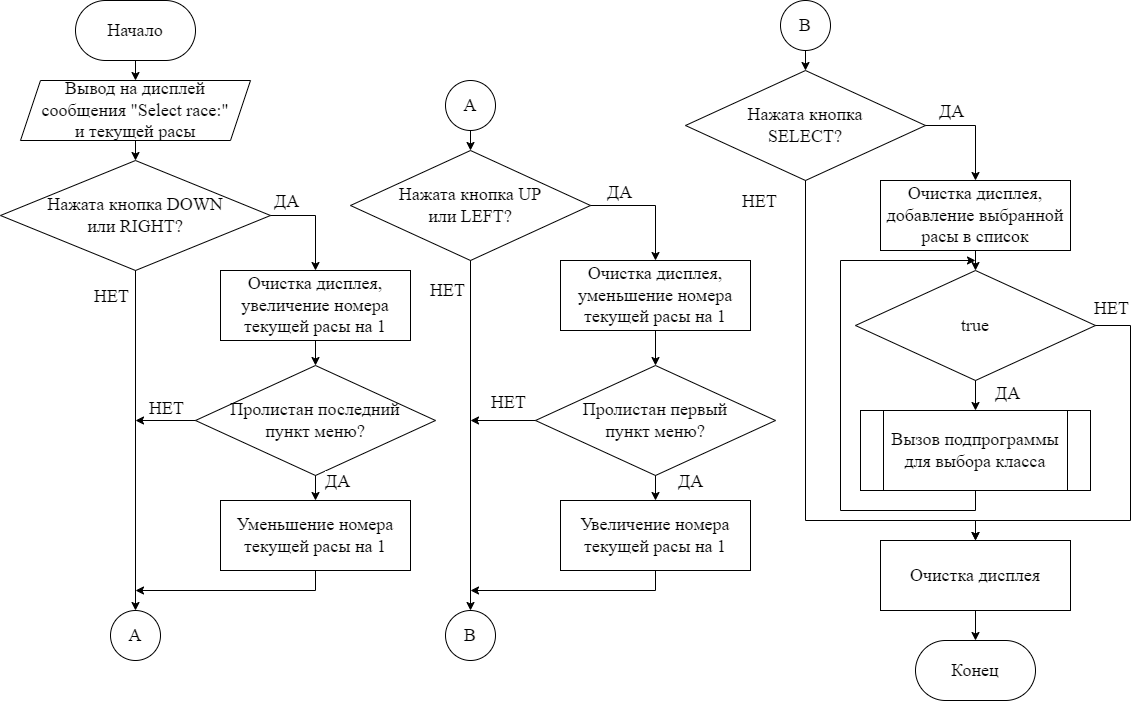
\includegraphics[width=\textwidth]{racePers.png}
        \label{fig:racePers}
    \end{figure}
\end{frame}

\newlength\someheight
\setlength\someheight{3,5cm}

\begin{frame}[fragile]{{\small Code block for choosing a character race}}
    \begin{adjustbox}{width=\textwidth,height=\someheight,keepaspectratio}
    \begin{minipage}{1.1\linewidth}
    \begin{minted}{C++}
        if(i == 0) {    //  Верхний пункт меню
            lcd.print("Select race:");
            lcd.setCursor(0, 1);
            lcd.print(racePers[i]);
            lcd.createChar(2, arrowDown);
            lcd.setCursor(15, 1);
            lcd.print(char(2));
        } else if(i == 11) {    //  Нижний пункт меню
            lcd.print("Select race:");
            lcd.setCursor(0, 1);
            lcd.print(racePers[i]);
            lcd.createChar(1, arrowUp);
            lcd.setCursor(15, 0);
            lcd.print(char(1));
        } else {    //  Промежуточные пункты меню
            lcd.print("Select race:");
            lcd.setCursor(0, 1);
            lcd.print(racePers[i]);
            lcd.createChar(1, arrowUp);
            lcd.setCursor(15, 0);
            lcd.print(char(1));
            lcd.createChar(2, arrowDown);
            lcd.setCursor(15, 1);
            lcd.print(char(2));
        }
        delay(150);
        //  Обработка нажатия кнопок
        int btnRacePers = clickButton();
        switch (btnRacePers){
            case BTN_R:   //  Обработка нажатия кнопки RIGHT
                lcd.clear();
    \end{minted}
    \end{minipage}
    \hfill
    \begin{minipage}{1.1\linewidth}
    \begin{minted}{C++}
            i++;
            if (i > 11)
              i--;
            break;
          case BTN_U:   //  Обработка нажатия кнопки UP
            lcd.clear();
            i--;
            if (i < 0)
              i++;
            break;
          case BTN_D:   //  Обработка нажатия кнопки DOWN
            lcd.clear();
            i++;
            if (i > 11)
              i--;
            break;
          case BTN_L:   //  Обработка нажатия кнопки LEFT
            lcd.clear();
            i--;
            if (i < 0)
              i++;
            break;
          case BTN_S:   //  Обработка нажатия кнопки SELECT
            pers[0] = racePers[i];  //Запоминаем выбранную расу
            lcd.clear();
            while(true) {
              lcd.home();
              genClassPers(); //Вызываем функцию выбора класса
            }
            break;
          default:
            break;
          }
          lcd.clear();
    \end{minted}
    \end{minipage}
    \end{adjustbox}
\end{frame}

\begin{frame}[fragile]{{\small Code block for choosing a character class}}
    \begin{adjustbox}{width=\textwidth,height=\someheight,keepaspectratio}
    \begin{minipage}{1.1\linewidth}
    \begin{minted}{C++}
        if(j == 0) {    //  Верхний пункт меню
          lcd.print("Select class:");
          lcd.setCursor(0, 1);
          lcd.print(classPers[j]);
          lcd.createChar(2, arrowDown);
          lcd.setCursor(15, 1);
          lcd.print(char(2));
        } else if(j == 12) {    //  Нижний пункт меню
          lcd.print("Select class:");
          lcd.setCursor(0, 1);
          lcd.print(classPers[j]);
          lcd.createChar(1, arrowUp);
          lcd.setCursor(15, 0);
          lcd.print(char(1));
        } else {    //  Промежуточные пункты меню
          lcd.print("Select class:");
          lcd.setCursor(0, 1);
          lcd.print(classPers[j]);
          lcd.createChar(1, arrowUp);
          lcd.setCursor(15, 0);
          lcd.print(char(1));
          lcd.createChar(2, arrowDown);
          lcd.setCursor(15, 1);
          lcd.print(char(2));
        }
        delay(150);
        //  Обработка нажатия кнопок
        int btnClassPers = clickButton();
        switch (btnClassPers){
          case BTN_R:   //  Обработка нажатия кнопки RIGHT
            lcd.clear();
    \end{minted}
    \end{minipage}
    \hfill
    \begin{minipage}{1.1\linewidth}
    \begin{minted}{C++}
            j++;
            if (j > 12)
              j--;
            break;
          case BTN_U:   //  Обработка нажатия кнопки UP
            lcd.clear();
            j--;
            if (j < 0)
              j++;
            break;
          case BTN_D:   //  Обработка нажатия кнопки DOWN
            lcd.clear();
            j++;
            if (j > 12)
              j--;
            break;
          case BTN_L:   //  Обработка нажатия кнопки LEFT
            lcd.clear();
            j--;
            if (j < 0)
              j++;
            break;
          case BTN_S:   //  Обработка нажатия кнопки SELECT
            pers[1] = classPers[j];
            lcd.clear();
            while(true) {
              lcd.home();
              charactPers();
            }
            break;
          default:
            break;
        }
        lcd.clear();
    \end{minted}
    \end{minipage}
    \end{adjustbox}
\end{frame}

\begin{frame}[fragile]{{\small Code block for generating the basic characteristics of the character}}
\begin{columns}
\begin{column}{0.35\textwidth}
\tiny
\begin{minted}[linenos,breaklines]{C++}
randomSeed(millis());
for (int i = 0; i < 6; i++) {
    roll = 6;
    characteristic = 0;
    for (int j = 0; j < 4; j++) {
        randRoll = random(1, 7);
        if (randRoll < roll) {
            roll = randRoll;
            characteristic += randRoll;
        } else {
            characteristic += randRoll;
        }
    }
    characteristics[i] = characteristic - roll;
}
\end{minted}
\end{column}
\begin{column}{0.65\textwidth}
    \begin{center}
     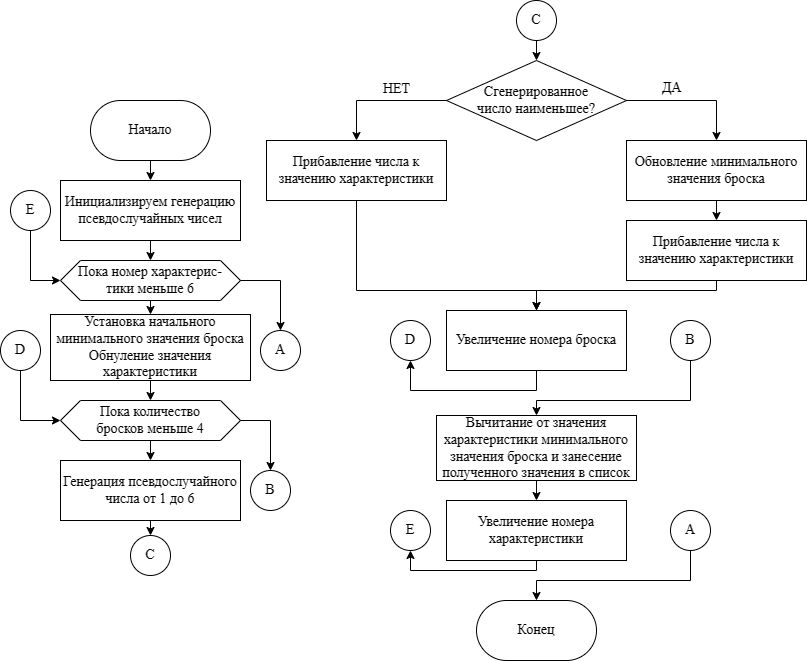
\includegraphics[width=\textwidth]{generate_character.png}
     \end{center}
\end{column}
\end{columns}
\end{frame}

\begin{frame}{The cost of components}
    \setlength{\parindent}{0.5cm}
    The following components were used to create a prototype:
    \begin{itemize}
        \item Arduino Uno --- 1200 rubles;
        \item LCD Keypad Shield --- 860 rubles.
    \end{itemize}

    The total cost of the components was: 2060 rubles.

     The cost of components separately:

    \begin{itemize}
        \item ATmega 328 --- 162 rubles;
        \item LCD-display 1602 --- 280 rubles;
        \item buttons --- 8 rubles for 1 thing.
    \end{itemize}
\end{frame}

\begin{frame}{Conclusion}
    \setlength{\parindent}{0.5cm}
    In the course of the work, the following tasks were solved:

    \begin{enumerate}
        \item еhe components necessary for prototyping of the characters genera-\ tor are selected;
        
        \item the functionality of the application is designed;
        
        \item implemented in the software code algorithms according to the basic rules D\&D5;
        
        \item the operability of the software and hardware part of the prototype of the device has been debugged and tested;
        
        \item the prototype of the device is assembled.
    \end{enumerate}
    
    As a result of the work, the device was designed and developed for generating the character D\&D and all assigned tasks were solved in full.
\end{frame}

\begin{frame}
    \centering Thank you for attention!
\end{frame}

% \begin{frame}{Немного о Dungeons \& Dragons}
%     \setlength{\parindent}{0.5cm}
%     Основной целью игры Dungeons \& Dragons является описание персонажа и его приключений. Для создания персонажа могут быть задействованы игральные кости и Основные правила, а также личные предпочтения игроков.

%     Основным средством для описания персонажа  служит лист персонажа -- сгруппированный в удобном виде набор характеристик персонажа. К таким характеристикам относятся следующие:

%     \begin{enumerate}
%         \item Основные атрибуты, присущие каждому персонажу: Сила, Телосложение, Ловкость, Интеллект, Мудрость, Харизма;
    
%         \item Особые умения, которые индивидуализируют персонажа: способность к убеждению или расследованию;
    
%         \item Определенные действия, такие как атака оружием или произнесение заклинаний;
    
%         \item Языки, на которых говорит персонаж, или инструменты, которыми он умеет пользоваться.
%     \end{enumerate}
% \end{frame}

% \begin{frame}{\smallПравила для генерации базовых характеристик персонажа}
%     \setlength{\parindent}{0.5cm}
%     Персонаж обладает шестью характеристиками: Сила, Телосложение, Ловкость, Интеллект, Мудрость и Харизма.
    
%     Есть несколько способов для генерации:

%     \begin{enumerate}
%         \item 3d6 -- классический способ, генерация осуществляется броском 3d6 (трёхкратным броском шестигранного кубика).

%         \item 4d6 -- один из альтернативных способов, генерация осуществляется броском 4d6 (четырехкратным броском игральной кости), а минимальное значение среди бросков отбрасывается.

%         \item Персонаж начинает со всеми характеристикам равными 8. У игрока есть 27 очков, которые он может свободно распределить, при этом 14 и 15 значение характеристики стоят по 2 очка каждое.

%         \item В D\&D 5e основной метод определения характеристик -- выбор из набора стандартных значений: 15, 14, 13, 12, 10, 8.
%     \end{enumerate}
% \end{frame}

% \begin{frame}{Выбор расы и класса персонажа}
%     \setlength{\parindent}{0.5cm}
%     Каждый персонаж принадлежит расе -- виду, в мире фэнтези. Самые общие игровые расы -- это дварфы, эльфы, халфлинги и люди. Существует еще много иных рас, которые могут быть доступны на усмотрение Мастера.
    
%     Раса персонажа, в частности определяет его расовые черты, такие как корректировка очков характеристик, особые чувства, талант к использованию определенного оружия, или способность использовать малые заклинания. Иногда эти черты соответствуют возможностям определенных классов.
    
%     Каждый персонаж также -- член класса. Самые распространенные классы -- это жрец, боец, разбойник и маг. Другие классы могут быть доступны на усмотрение Мастера.
    
%     Персонаж также получает некоторые преимущества от выбранного класса. Многие из этих преимуществ это особенности класса, отличающие его от остальных.
% \end{frame}
\end{document}
